\documentclass[a4paper]{article}

\usepackage[utf8]{inputenc}
\usepackage[russian]{babel}

\usepackage{a4wide,color,url,amsmath,amsthm,amssymb,booktabs,longtable,eurosym}
\newenvironment{question}{\item \textbf{Problem}\newline}{}
\newenvironment{solution}{\textbf{Solution}\newline}{}
\newenvironment{answerlist}{\renewcommand{\labelenumi}{(\alph{enumi})}\begin{enumerate}}{\end{enumerate}}
\providecommand{\tightlist}{\setlength{\itemsep}{0pt}\setlength{\parskip}{0pt}}

\DeclareMathOperator{\Cov}{Cov}
\DeclareMathOperator{\Corr}{Corr}
\DeclareMathOperator{\Var}{Var}
\DeclareMathOperator{\E}{E}
\let\H\relax
\DeclareMathOperator{\H}{H}
\def \hb{\hat{\beta}}
\def \hs{\hat{\sigma}}
\def \htheta{\hat{\theta}}
\def \s{\sigma}
\def \hy{\hat{y}}
\def \hY{\hat{Y}}
\def \v1{\vec{1}}
\def \e{\varepsilon}
\def \he{\hat{\e}}
\def \z{z}
\def \hVar{\widehat{\Var}}
\def \hCorr{\widehat{\Corr}}
\def \hCov{\widehat{\Cov}}
\def \cN{\mathcal{N}}

\let\P\relax
\DeclareMathOperator{\P}{\mathbb{P}}

\DeclareMathOperator{\plim}{plim}


\usepackage{hyperref}

\usepackage{graphicx}

\usepackage{float}

\begin{document}
\begin{enumerate}

\begin{question}
Consider a process \(y_t = 5 + 0.3 y_{t-1}\), where \(u_t\) is a white noise with variance 2.

Construct a point forecast 4 steps ahead given that \(y_T=2\).\\
Provide the answer with 3 decimal digits.
\end{question}

\begin{solution}
The point forecast will be equal to \(E(y_{t+4}\mid \mathcal{F}_t) = (1 + 0.3 + 0.3^2 + 0.3^3)*5+0.3^4*2\).
\end{solution}



\begin{question}
Consider a process \(y_t = -1 + u_t + 0.8 u_{t-1} - 0.4 u_{t-2}\), where \(u_t\) is a white noise with variance 4.

Construct an 95\% prediction interval 2 steps ahead, given that \(\hat{u}_T=0.5, \hat{u}_{T-1}=-0.3\).\\
Provide the variance of the point forecast rounded to 3 decimal digits as the answer.
\end{question}

\begin{solution}
The variance of the point forecast will be equal to \(Var(y_{t+2}\mid \mathcal{F}_t) = Var(u_{t+2} + 0.8 u_{t+1} \mid \mathcal{F}_t)\)
\end{solution}



\begin{question}
Suppose we have splitted time series into training and test sets and estimated three different models. Which of the following statements ARE correct?
\begin{answerlist}
  \item This approach can be preferred to a cross-validation if the dataset is small
  \item We cannot choose the best model using this method since forecasts have different horizons
  \item Since forecasts have different horizons we cannot differentiate models which are better for short-term forecasts and long-term forecasts
\end{answerlist}
\end{question}

\begin{solution}
\begin{answerlist}
  \item True.
  \item False. We certainly can!
  \item True.
\end{answerlist}
\end{solution}



\begin{question}
Which of the following is regressors should be chosen for modelling yearly seasonality in daily data?
\begin{answerlist}
  \item Either \(\operatorname{cos}\left({\frac{2\pi}{365}}\cdot\,t\right)\) or \(\operatorname{sin}\left({\frac{2\pi}{365}}\cdot\,t\right)\)
  \item 365 dummies for each day of the year
  \item Both \(\operatorname{cos}\left({\frac{2\pi}{365}}\cdot\,t\right)\) and \(\operatorname{sin}\left({\frac{2\pi}{365}}\cdot\,t\right)\)
\end{answerlist}
\end{question}

\begin{solution}
\begin{answerlist}
  \item Check lecture ``More predictors''.
  \item NA
  \item NA
\end{answerlist}
\end{solution}



\begin{question}
Consider gas dataset. You need to do STL with 2 inner and 1 outer loop for log(gas). Calculate the strength of trend using the practical formula for the first 12 years of observations and for the last 12 years. Give the absolute value of the difference between them as an answer. Provide the answer rounded up to 4 decimal digits.

You can load the gas dataset in R by importing forecast library or if you use other programming languages you can download it \href{https://github.com/vincentarelbundock/Rdatasets/blob/master/csv/forecast/gas.csv}{here}.
\end{question}

\begin{solution}
Calculate strength of trend according to the formulas given in the lecture.
\end{solution}



\begin{question}
Consider the following ARMA equation \(y_t= 0.4 y_{t-1} + 0.45 y_{t-2} + u_t + u_{t-1}+ 0.25 u_{t-2}\), where \(u_t\) is a white noise with variance 1. Which of the following is true?
\begin{answerlist}
  \item The process is non-invertible
  \item The ARMA equation has a unique solution
  \item The equation is irreducible
  \item The corresponding ARMA process satisfying the is stationary
\end{answerlist}
\end{question}

\begin{solution}
There is one common factor, hence in fact it is an ARMA(1,1). If you check the roots for this reduced process, it will be clear the process is stationary and invertible.
\end{solution}



\begin{question}
Consider gas dataset. You need to do STL with 2 inner and 1 outer loop for log(gas). Next check whether the variance of the first half of the seasonal component equals to the second using F-test. Provide the p-value rounded up to 2 decimal digits.

You can load the gas dataset in R by importing forecast library or if you use other programming languages you can download it \href{https://github.com/vincentarelbundock/Rdatasets/blob/master/csv/forecast/gas.csv}{here}.
\end{question}

\begin{solution}
You can use var.test(x, y, alternative = ``two.sided'').
\end{solution}



\begin{question}
Which of the following statements are true?
\begin{answerlist}
  \item You can improve forecast quality by averaging forecasts of a complex model and a naive one.
  \item There is no model to approximate dynamics of non-stationary time series.
  \item You can model stationary process using random walk model.
  \item A very complex model can perform worse than a naive independent observations model.
\end{answerlist}
\end{question}

\begin{solution}
\begin{answerlist}
  \item True.
  \item False. The stationary series models are similar to the independent observations model; non-stationary series models are similar to a random walk.
  \item False. The stationary series models are similar to the independent observations model; non-stationary series models are similar to a random walk.
  \item True.
\end{answerlist}
\end{solution}



\begin{question}
Which of the following statements ARE correct?
\begin{answerlist}
  \item MAPE can be used to compare models performances between datasets
  \item IF MASE is greater than 1 then a naive model is better
  \item For SMAPE if the actual value or forecast value is 0, the value of error will approach 100\%
  \item RMSE is robust to outliers
\end{answerlist}
\end{question}

\begin{solution}
\begin{answerlist}
  \item True.
  \item False. IF MASE is greater than 1 then a naive model is worse
  \item True.
  \item False. RMSE is sensitive to outliers
\end{answerlist}
\end{solution}



\begin{question}
Consider a process \(y_t = 4 + 0.8 y_{t-1} + u_t\), where \(u_t\) is a white noise with variance 3.

Find it's autocovariance function \(\gamma_k\). Give \(\gamma_0\) as an answer. Provide the answer with 3 decimal digits.
\end{question}

\begin{solution}
You are need to find the variance of \(y_t\). Note, that the process is stationary, so its variance does not change over time.
\end{solution}



\begin{question}
Match ACF and PACF with their corresponding ARMA processes:

\textit{Picture A}

\textit{Picture B}

\textit{Picture C}

\textit{Picture D}

\begin{enumerate}
\def\labelenumi{\arabic{enumi}.}
\item
  ARMA(2,0)
\item
  ARMA(1,0)
\item
  ARMA(1,2)
\item
  ARMA(0,2)
\end{enumerate}

Write down in the solution the sequence of numbers without spaces or delimeters corresponding to pairs of ACF and PACF in each case (e.g.~4231).
\end{question}

\begin{solution}
A gradual geometrically declining ACF and a PACF that is significant for only a few lags indicate an AR process. MA process shows a gradually geometrically declining PACF and the ACF has a few significant lags. An ARMA process is indicated by geometrically filling ACF and PACF.
\end{solution}



\begin{question}
Select all of the assumptions for ARMAX model

\[y_t = c + \gamma a_t +  \beta_1 y_{t-1} + \ldots + \beta_p y_{t-p}  + u_t + \alpha_1 u_{t-1} + \ldots + \alpha_q u_{t-q }\]

where \(a_t\) is a predictors and \((u_t)\) is white noise
\begin{answerlist}
  \item \(E(a^4_t) < \infty\)
  \item Series \((y_t)\) is non-stationary
  \item Predictor \((a_t)\) is stationary
  \item \(E(u_t \mid a_{t-1}, b_{t-1}, y_{t-1}, a_{t-2}, b_{t-2}, y_{t-2} , \ldots) = 0\)
  \item Predictor \((a_t)\) is non-stationary, but \(\Delta(a_t)\) is stationary
  \item Series \((y_t)\) is stationary
\end{answerlist}
\end{question}

\begin{solution}
\begin{answerlist}
  \item True.
  \item False. \((y_t)\) and \((a_t)\) should be stationary
  \item True.
  \item True.
  \item False. \((y_t)\) and \((a_t)\) should be stationary
  \item True.
\end{answerlist}
\end{solution}



\begin{question}
Consider gas dataset. You need to use seasonal naive model to forecast gas production one year ahead. Calculate the width of prediction interval 2 and 12 steps ahead. Give the absolute value of the difference of these widths as an answer.

You can load the gas dataset in R by importing forecast library or if you use other programming languages you can download it \href{https://github.com/vincentarelbundock/Rdatasets/blob/master/csv/forecast/gas.csv}{here}.
\end{question}

\begin{solution}
Check lecture ``Naive models''.
\end{solution}



\begin{question}
Consider gas dataset. You need to estimate an ARIMA and ETS model with automatically chosen parameters. Compare out-of-sample forecasts 6 steps ahead using MAPE. Provide MAPE for the best of the compared models with 3 decimal digits as an answer.

You can load the LakeHuron data set in R by issuing the following command at the console data(``LakeHuron'') or if you use other programming languages you can download it \href{https://github.com/vincentarelbundock/Rdatasets/blob/master/csv/datasets/LakeHuron.csv}{here}.
\end{question}

\begin{solution}
You can use dm.test(residuals(f1),residuals(f2),h=1) function.
\end{solution}



\begin{question}
Consider a process \(y_t = 2 + u_t + 0.2 u_{t-1} - 0.2 u_{t-1}\), where \(u_t\) is a white noise with variance 5.

Check that the process is invertible. If the process is invertible give the sum of the characteristic polynomial roots as an answer, else give 0 as an answer.
Provide the answer with 3 decimal digits.
\end{question}

\begin{solution}
The process is invertible.
\end{solution}



\begin{question}
Let's conduct a Box-Jenkins procedure for gas time series to determine the specification of SARIMA model.

You can load the gas dataset in R by importing forecast library or if you use other programming languages you can download it \href{https://github.com/vincentarelbundock/Rdatasets/blob/master/csv/forecast/gas.csv}{here}.

\begin{figure}[H]
\centering
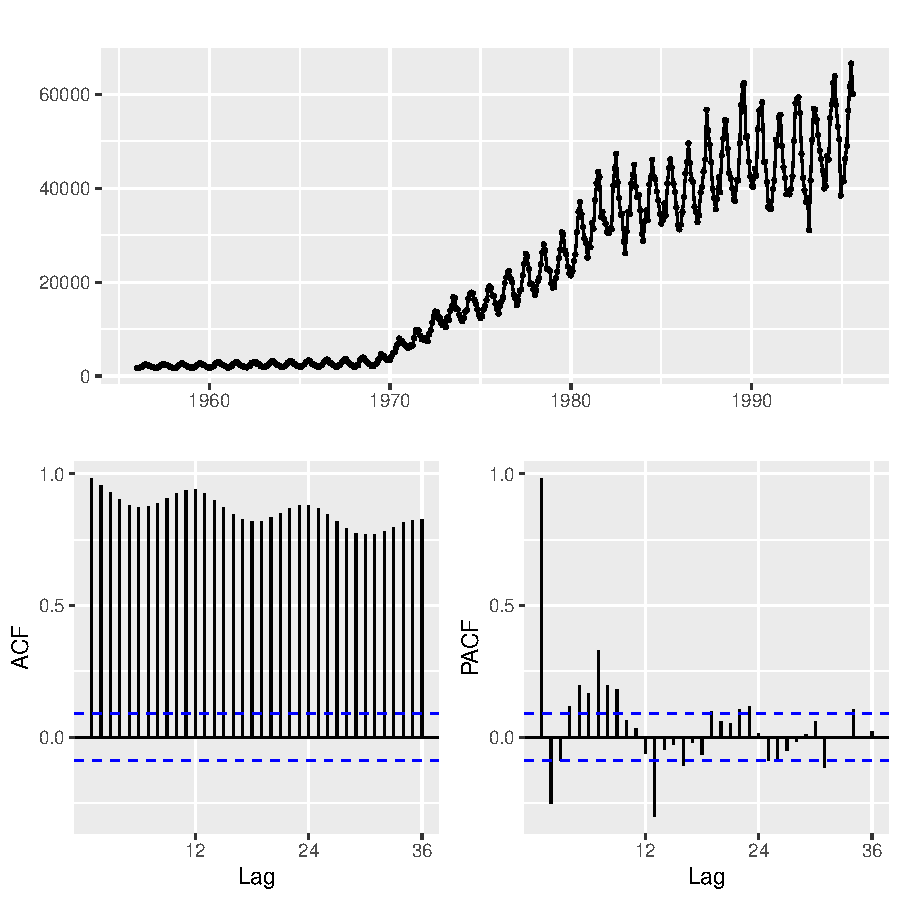
\includegraphics{unnamed-chunk-1-1-4.pdf}
\caption{plot of chunk unnamed-chunk-1}
\end{figure}

Is the variance stable?
\begin{answerlist}
  \item Yes, we can proceed with gas time series
  \item No, the logarithmic transformation should be applied
\end{answerlist}
\end{question}

\begin{solution}
The variance grows over time, a transformation is required.
\end{solution}



\begin{question}
Consider ETS(AAdN) model with \(\ell_0 = 90, b0 = 10, \phi=0.9, \alpha=0.1,\beta=0.2,\sigma^2=10\). We know that \(y_1=100\).

Find smoothed value \(\ell_1\).

Provide the answer with 2 decimal digits.
\end{question}

\begin{solution}
Plug everything in a model and derive \(\ell_1\).
\end{solution}



\begin{question}
What is correct about LOESS?
\begin{answerlist}
  \item You can only use normal Kernel function
  \item The bigger the window \(h\) the smoother the resulting curve
  \item You can predict using LOESS
  \item The higher the degree of the polynomial the smoother the resulting curve
\end{answerlist}
\end{question}

\begin{solution}
\begin{answerlist}
  \item False. You can use any kernel function
  \item True.
  \item True.
  \item False. It works other way around
\end{answerlist}
\end{solution}



\begin{question}
Consider gas dataset. Estimate ETS model without a trend and automatically selected error and seasonality specification. Calculate point forecast 2 years ahead. Provide the answer with 2 decimal digits.

You can load the gas dataset in R by importing forecast library or if you use other programming languages you can download it \href{https://github.com/vincentarelbundock/Rdatasets/blob/master/csv/forecast/gas.csv}{here}.
\end{question}

\begin{solution}
You can use ets(x,``ZZZ'') function.
\end{solution}



\begin{question}
Consider gas dataset. You need to estimate a linear regression model for the logarithm of gas series staring from 1970. Use square root of the trend as a regressor. Provide the forecast 10 steps ahead for the log(gas) rounded up to 3 decimal digits as an answer.

You can load the gas dataset in R by importing forecast library or if you use other programming languages you can download it \href{https://github.com/vincentarelbundock/Rdatasets/blob/master/csv/forecast/gas.csv}{here}.
\end{question}

\begin{solution}
You can use lm() and predict() functions.
\end{solution}



\begin{question}
Consider a seasonal random walk model for the following sample \(y^T = [1, 3, 2, -1, 2, 4, 2, -3]\) of quarterly observations. Construct a 95\% prediction interval 19 steps ahead. Provide upper margin of thw interval as the answer.

Provide the answer with 2 decimal digits.
\end{question}

\begin{solution}
Check lecture ``Naive models''.
\end{solution}



\begin{question}
Consider LakeHuron dataset. You need to calculate how many lags in ACF are significant.

You can load the LakeHuron data set in R by issuing the following command at the console data(``LakeHuron'') or if you use other programming languages you can download it \href{https://github.com/vincentarelbundock/Rdatasets/blob/master/csv/datasets/LakeHuron.csv}{here}.
\end{question}

\begin{solution}
Use acf(x, plot = FALSE) function.
\end{solution}



\begin{question}
Consider the process \(x_t = 0.5 x_{t−1} + 2 u_{t−1} + u_{t}\), where \(u_t\) is a white noise process.
\begin{answerlist}
  \item non-invertible and stationary
  \item invertible and stationary
  \item invertible and non-stationary
  \item non-invertible and non-stationary
\end{answerlist}
\end{question}

\begin{solution}
Non-invertible since root of MA polynomial is not outside unit circle.
Non-stationary, since root of AR polynomial is outside unit circle.
\end{solution}



\begin{question}
Consider ARDL model

\[y_t = c+  \beta_1 y_{t-1} + \ldots + \beta_p y_{t-p} + x_t + \alpha_1 x_{t-1} + \ldots + \alpha_q x_{t-q }  + u_t. \]

Which of the following statements about ARDL model ARE correct?
\begin{answerlist}
  \item ARDL model can be used if you want to find a long-term relationships between time series
  \item ARDL model can model non-stationary \(y_t\)
  \item \((u_t)\sim ARMA(p,q)\) w.r.t. white noise
  \item ARDL model allows only one predictor for \(y_t\)
\end{answerlist}
\end{question}

\begin{solution}
\begin{answerlist}
  \item Check lecture about prediction with AR type models
  \item NA
  \item NA
  \item NA
\end{answerlist}
\end{solution}


\end{enumerate}
\end{document}
